\section{Interface Descriptions}

\begin{wrapfigure}{r}{0.25\textwidth}
	\vspace{-25pt}
	\begin{center}
	
\includegraphics[width=0.18\textwidth]{images/flags_greye}
	\caption{The available (left) and unavailable (right) place cache button.}
	\label{flags_greye}
	\end{center}
	\vspace{-10pt}
\end{wrapfigure}

The design of a good user interface is key to a successful system, playing a vital role in attracting users. Indeed Douglas Bell (1987:GETPAGENUMBERPLEASE) stated that the user interface is the ``yardstick by which a system is judged''. This section will describe how the final product will be suitable, appealing and fulfil the criteria in the requirements document (23 Cats, 2012).
\vspace{-10pt}

\subsection{Design Methodology}
\subsubsection{Fortitude Application}

\begin{wrapfigure}{l}{0.25\textwidth}
	\vspace{-20pt}
	\begin{center}
	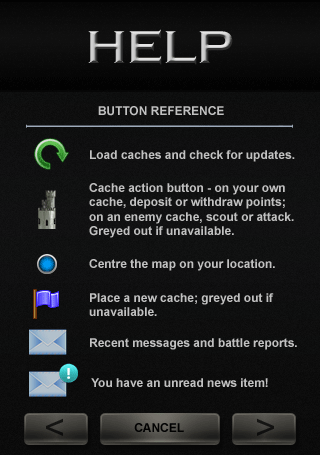
\includegraphics[width=0.25\textwidth]{images/help_mockup}
	\caption{Button reference in the help section.}
	\label{help_mockup}
	\end{center}
	\vspace{-20pt}
\end{wrapfigure}

Our design is easy to use for users of various levels of familiarity with the system. The domain analysis showed us the significance of intuitiveness and easy accessibility (23 Cats, 2012:5-7); therefore we have designed a clear interface with a help screen (see fig \ref{help_mockup}). Bell (1987) says a well designed user interface reduces errors so we have tested many features of the app on potential users during development. In particular, it had been decided to disable the android back button to give the implementers greater control over which screens the user could access at any point in time. This proved difficult for users to adapt to, so instead the back button was incorporated into the application.

To further ease of use, buttons will be greyed out when their action is not available and will perform no function. For example when a user is too close to an existing cache the `place cache' button will be greyed out (see fig \ref{buttons}).

The application's screens satisfy requirement 5.3.7: Interface Style Uniformity by their colour scheme and placement of buttons and headers. The colour scheme is silver or white on black, as this is easily read, even by people who are colour blind. The app provides a fast response to user input by using separate images for on-press actions ensuring the system has received the user's request (see fig \ref{website_header_background}), which satisfies requirement 5.3.9: Interface Feedback Delay.

\begin{figure}[ht]
	\vspace{-10pt}
	\begin{center}
	
\includegraphics[width=0.3\textwidth]{images/buttons}
	\vspace{-10pt}
	\caption{An inactive button (left) and an active button (right).}
	\label{buttons}
	\end{center}
\end{figure}

\subsubsection{Fortitude-game.co.uk Website}

\begin{figure}[ht]
	\begin{center}
	
\includegraphics[width=0.9\textwidth]{images/website_header_background}
	\caption{The header image, an example of the more complex graphics used in the website. The white bordered box will hold the navigation.}
	\label{website_header_background}
	\end{center}
	\vspace{-20pt}
\end{figure}

\begin{wrapfigure}{r}{0.25\textwidth}
	\vspace{-15pt}
	\begin{center}
	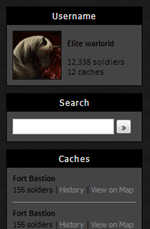
\includegraphics[width=0.25\textwidth]{images/sidebar_modules}
	\caption{Examples of the individual `modules' that comprise the website (in this instance, the sidebar).}
	\label{sidebar_modules}
	\end{center}
	\vspace{20pt}
\end{wrapfigure}

There is a website to support the Fortitude application. With its larger dimensions and lack of battery and data restrains, the website can provide functionality not feasible with the application, such as requirement 5.3.6: Activity Recording. This means the app can be simpler, and therefore more user friendly without compromising the scope of the system.
Through the website, administrators can interact with app as specified by many requirements including 5.1.3: Administrator Accounts. This is an easy to access alternative to bespoke software, and is not device dependant so administrators can perform all actions without an Android device.
The website design matches the application design by using the same colour scheme, recognisable logo of two flags flying over a castle tower and a navigation menu that echoes the message box of the app, which satisfies requirement 5.4.8: Website Application Style Uniformity. However the design has been expanded upon in the website to be more visually appealing, while these graphics could not be included in the app without sacrificing ease of use.

\begin{wrapfigure}{r}{0.3\textwidth}
	\vspace{-20pt}
	\begin{center}
	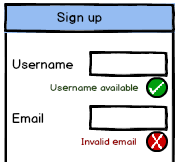
\includegraphics[width=0.25\textwidth]{images/sign_up_wireframe}
	\caption{Wireframe showing user feedback when creating an account.}
	\label{sign_up_wireframe}
	\end{center}
	\vspace{-50pt}
\end{wrapfigure}

Commonly accessed areas of the website, such as the sidebar and the homepage, are organised into modules (see fig \ref{fig:sidebar_modules}), making information quickly and easily identifiable. It also provides an excellent template for adaption; though out of scope for this project, users could in future personalise the website by selecting which modules to display.

The website provides feedback, by validating data (see \ref{fig:sign_up_wireframe}) or by providing loading messages, so the user can interact efficiently and with fewer errors. For more critical data entry, such as an administrator creating a new cache, the user is presented with a summary page of the information they have entered and must confirm it is correct before the new data is stored.

The website also provides feedback if an error occurs - the most common anticipated is the user having javascript disabled. This will cause every javascript dependent element of the site to be replaced with a placeholder of the correct shape to avoid disturbing the website layout which informs the user that javascript is required.

\subsection{Process Descriptions}
\subsubsection{Opening the application}

The process of opening the application will be quick and efficient. Therefore the user will be taken straight to the main screen from the splash screen if they are already signed into the application.

Users who have not activated their accounts are given limited functionality while using the application, which fulfils requirement 5.1.2: Account activation. The screen to create a new user leads directly to the unactivated main screen; and the user can get to the activated main screen when they open the app after activating their account through the verification email sent to them. As per requirement 5.1.4: Resend activation email, the user can request a new activation email from the unactivated main screen.

\begin{figure}[h!]
\centering
\begin{tabular}{cc}
	\begin{minipage}{0.4\textwidth}
		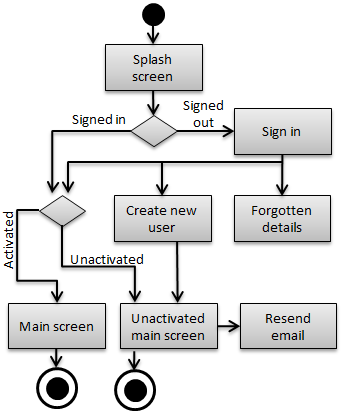
\includegraphics[width=1\textwidth]{images/opening_app}
		\caption{Screen map for the process of opening the app.}
		\label{opening_app}
	\end{minipage}
	\begin{minipage}{0.5\textwidth}
		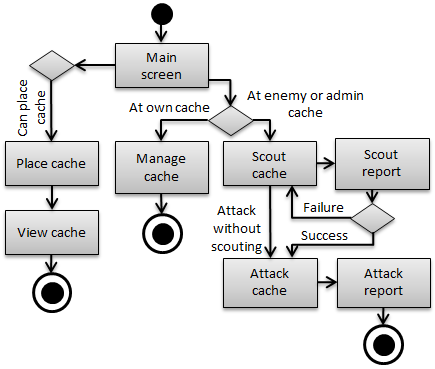
\includegraphics[width=1\textwidth]{images/key_actions}
	\caption{Screen map for key game actions.}
	\label{key_actions}
	\end{minipage}
\end{tabular}
\vspace{-20pt}
\end{figure}

\newpage
\subsubsection{Performing key game actions}

The key actions to Fortitude game play are creating caches (place cache), defending caches (manage cache) and conquering caches (scout then attack cache), which are all accessible through the main screen. These actions require the user to be at the cache or cache they want to place, otherwise the buttons will be greyed out (see fig 2.2). The same button is used to manage a cache (deposit or withdraw defending troops, or abandon the cache by withdrawing all troops) and attack an enemy cache. This simplifies the process of playing the game for the user and reduces redundancy and clutter on the main screen.

\subsubsection{Viewing caches}

\begin{wrapfigure}{r}{0.5\textwidth}
	\vspace{-20pt}
	\begin{center}
	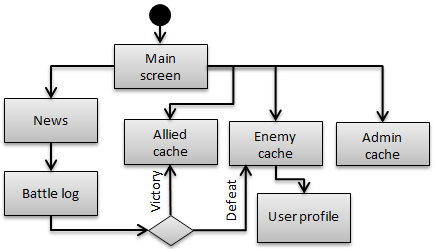
\includegraphics[width=0.5\textwidth]{images/viewing_caches}
	\caption{Screen map for key game actions.}
	\label{viewing_caches}
	\vspace{-20pt}
	\end{center}
\end{wrapfigure}

Viewing caches is integral to the above actions and can be done from the main screen (see fig 2.15) whether or not the user is at the cache. This allows the user to plan strategies, keep track of their caches and plan routes to caches displayed on the map (see fig 2.14), which satisfies requirement 5.3.4: Path finding. The user can also view a profile of an enemy through their cache and report the cache to admins (see fig 2.2.5).

After a user's cache is attacked, they can see the battle report from their notifications and then view the cache. If their defenders were victorious, they will see an allied cache, but if the attackers won they will see an enemy cache.

\subsubsection{Reading and sending messages}

\begin{wrapfigure}{r}{0.4\textwidth}
	\vspace{-20pt}
	\begin{center}
	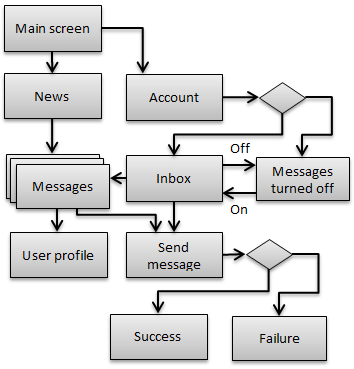
\includegraphics[width=0.4\textwidth]{images/sending_messages}
	\caption{Screen map for the messaging system.}
	\label{sending_messages}
	\end{center}
	\vspace{-20pt}
\end{wrapfigure}

Users can interact with each other by sending messages, allowing alliances and battle strategies to be formed and satisfying requirement 5.4.1: User communication. From the inbox, users are given the option to turn the messaging system off. If, due to this or any other reason, a user can not send a message then they will be informed through a `Failure' screen. This is so a user is informed and won't send multiple messages believing the previous ones have failed. Users can also report communications and block users (see 2.2.5).

Requirements 5.2.2: Cache reporting and 5.4.2: Communication reporting both require the user to be able to alert the administrators of certain caches or communications. This is anticipated to include a cache placed on a private or otherwise inaccessible location, or users behaving inappropriately towards others, and will be handled through a single report form (fig 2.8). The subject line is automatically filled in according to the screen from which the user reported from (see fig 2.9), and a copy of the offending message, user profile or cache is sent with the body of the report that gives administrators as much information as possible.

\begin{figure}[ht]
	\begin{minipage}{0.5\textwidth}
	\begin{tabularx}{\textwidth}{| X | X |}
		\hline
		Outlaw camp & Outlaw camp \\
		Enemy cache & User owned cache \\
		Allied cache & User owned cache \\
		Message & User communication \\
		User profile & User profile \\
		\hline
	\end{tabularx}
	\caption{Screens from which a user can report,
	and the corresponding subject line.}
	\label{report_table}
	\end{minipage}
\end{figure}

\begin{wrapfigure}{r}{0.25\textwidth}
	\vspace{-180pt}
	\begin{center}
	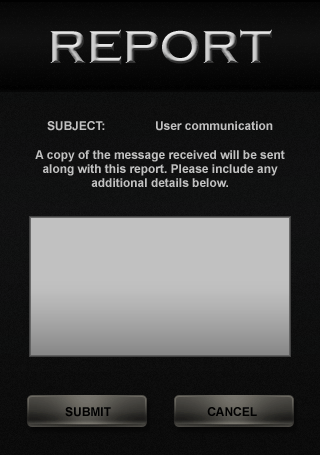
\includegraphics[width=0.25\textwidth]{images/report_mockup}
	\caption{Mock-up of the report screen.}
	\label{report_mockup}
	\end{center}
	\vspace{-60pt}
\end{wrapfigure}

Blocking users stops the user who blocks from receiving messages from the users they have blocked. From their inbox, a user can see a list of blocked users, block and unblock users. Blocking can be done from the user profile too.

\subsubsection{Administrators acting on user request}
\subsubsection{Reporting and Blocking}

User requests from the app are always in the form of a report as detailed in 2.2.5. A user may submit other requests from the website, including a request to delete their account or a support question sent through the help page. All of these requests must be acted upon by an administrator through the admin section of the website. When a user deletes their account they must confirm their action through an email sent to them before the request is sent to the administrators.

\newpage
\begin{wrapfigure}{r}{0.4\textwidth}
	\vspace{-20pt}
	\begin{center}
	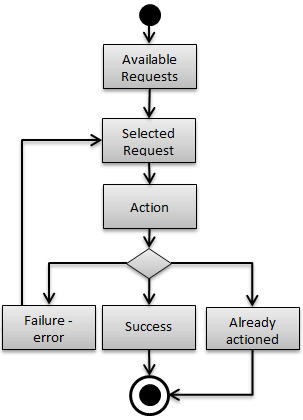
\includegraphics[width=0.33\textwidth]{images/admins_acting}
	\caption{Administrators acting on a user request.}
	\label{admins_acting}
	\end{center}
	\vspace{-20pt}
\end{wrapfigure}

On the website, administrators are able to see a page of all user requests not being worked on by another administrator. The administrator selects a request, which removes it from the requests page, and performs an action on it to complete the request or flag it if it can't be dealt with by that administrator at that time. The administrator will be informed of the result of their action and any details about a failure, such that the administrator can correct their mistake or flag the request. In the unlikely event that two administrators try to action the same request, the first action will be performed and the second administrator informed of this when they submit their own action. Once acted upon, requests will be accessible through a `past requests' page.

\subsubsection{Miscellaneous other}

\begin{wrapfigure}{r}{0.25\textwidth}
	\vspace{-60pt}
	\begin{center}
	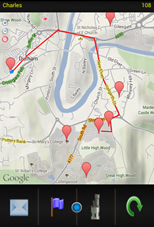
\includegraphics[width=0.25\textwidth]{images/route_mapping}
	\caption{Displaying a route to a cache.}
	\label{route_mapping}
	\end{center}
	\vspace{-30pt}
\end{wrapfigure}

A user can sign out from the user account settings, accessed from clicking on the status bar on the main screen.

Special placement caches appear on the screen if the user has the application open at the correct location. They can then choose to accept or reject the award for finding the cache.

Routes to caches are shown on the main map as a thick red line (see fig 2.14). They can be planned from `view cache' screens, and cleared in the account menu. As routes are cleared before a new one is made only one route can be displayed on the map at once.
\vspace{30pt}

\subsection{User Interface Design - Fortitude Application}

\subsubsection{Main screen}

\begin{wrapfigure}{l}{0.25\textwidth}
	\vspace{-20pt}
	\begin{center}
	
\includegraphics[width=0.25\textwidth]{images/news_icons}
	\caption{The `Recent news' icon and (right) with notification.}
	\label{news_icons}
	\end{center}
	\vspace{-20pt}
\end{wrapfigure}

\begin{figure}[ht]
	\begin{center}
	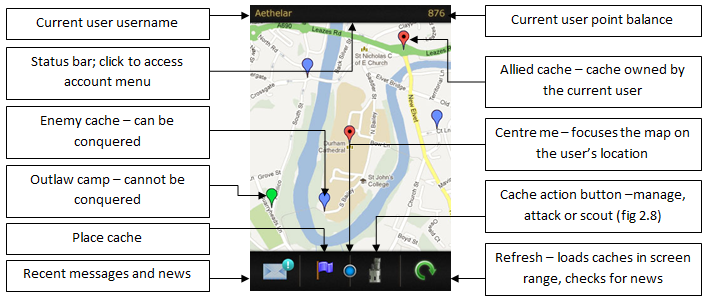
\includegraphics[width=0.9\textwidth]{images/main_screen}
	\caption{The main screen of the Fortitude application.}
	\label{main_screen}
	\end{center}
\end{figure}

The main screen is the core of the Fortitude application through which all key features are easily accessible. These are split into features relating to playing the game, grouped in the action bar at the bottom of the screen, and features relating to providing the user with information or allowing them to access their account, grouped in the status bar at the top of the screen. When clicked, this status bar leads the user to their account menu through which they can sign out, access their message inbox, or view the help screen. The status bar also displays the point balance available to the user; as points are required for core actions, it is important that this information is very visible, as specified by functional requirement 5.2.1: Account balance.

The action buttons relating to game play are grouped at the bottom of the screen, where it is most ergonomic for the user to access them. Each button is clearly distinct and, where appropriate, contains easily discernible extra information - such as the place cache and cache action buttons being greyed out when unavailable (see fig 2.2) and the recent news having a notification symbol to indicate unread news (fig 2.16). 

\begin{wrapfigure}{l}{0.2\textwidth}
	\vspace{-20pt}
	\begin{center}
	
\includegraphics[width=0.15\textwidth]{images/grey_pins}
	\caption{The pins are easy to tell apart without colour.}
	\label{grey_pins}
	\end{center}
	\vspace{-20pt}
\end{wrapfigure}

The main area of the home screen is the map, chosen as a very user friendly interface for the game and fulfilling several requirements including 5.3.1: Display location and 5.2.3: Nearby caches. Caches are clearly distinguished with different coloured pins to differentiate between admin, allied and enemy caches, and allied caches further distinguished by the presence of a dot, as per requirement 5.2.3: Cache ownership and 5.2.26: Distinguishing cache owners; the colours are chosen to account for those with colour blindness (see fig 2.17). The map itself is controlled with the touch screen, using swipe or drag to navigate and pinch to zoom (zoom required by 5.3.3: Map zooming). To reduce data usage as per non-functional requirement 5.2.30: Data usage, adjusting the map view by zoom or location will not load the caches for that area of the map. This will be done by the green refresh arrow on the right of the status bar which also updates point balance, a route to a cache if active, and recent news feed as required.

\subsubsection{Unactivated main screen}

\begin{wrapfigure}{r}{0.25\textwidth}
	\vspace{-80pt}
	\begin{center}
	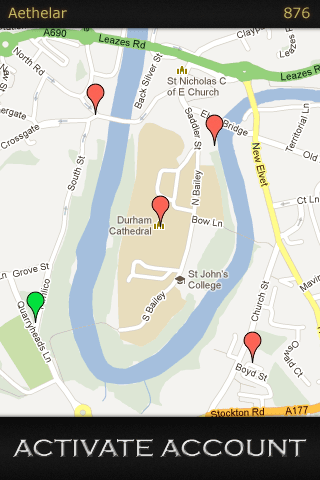
\includegraphics[width=0.25\textwidth]{images/unauthorised_main_mockup}
	\caption{Unactivated main screen.}
	\label{unactivated_main}
	\end{center}
	\vspace{-20pt}
\end{wrapfigure}

The main screen for the unactived user is identical in appearance to the main screen for an activated user (see fig 2.15), with the only difference being in the bottom bar. On the standard main screen this contains several buttons linking to features or actions which are not available to unactivated users - as specified by functional requirement 5.1.2: Account Activation. Here, this bar is replaced by a banner reminding users to activate their account; when clicked, this banner leads to the resend activation email page.

All other features have the same functionality as the main screen. The only difference is in navigating the map; on the unactivated account, each request to load a new view of the map also loads every cache within that view. This is because the unactivated user is not able to refresh the screen, as this button is located on the action bar which is not available here.

\subsubsection{User text input}

Many screens make use of text the user has input, most notably those involved with signing in or creating a new account (see fig 2.7) as well as sending messages to users (fig 2.19) or reports to administrators. Text input is handled through the on screen keyboard that is standard on an android phone (see fig 2.20). 
\vspace{0pt}
\begin{figure}[h!]
\centering
\begin{tabular}{cc}
	\begin{minipage}{0.3\textwidth}
		\begin{center}
		\begin{minipage}{0.83\textwidth}
		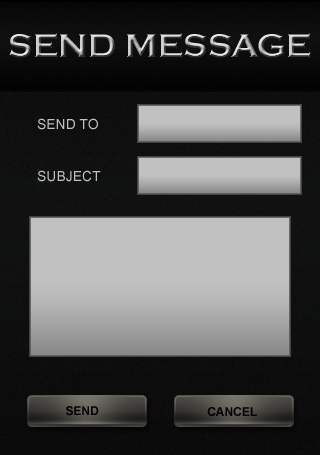
\includegraphics[width=\textwidth]{images/send_message_mockup}
		\caption{Send message screen, showing user text input fields.}
		\label{send_message}
		\end{minipage}
		\end{center}
	\end{minipage}
	\begin{minipage}{0.3\textwidth}
		\begin{center}
		\begin{minipage}{0.79\textwidth}
		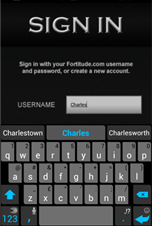
\includegraphics[width=\textwidth]{images/onscreen_keyboard}
		\caption{Using the on screen keyboard to sign in.}
		\label{onscreen_keyboard}
		\end{minipage}
		\end{center}
	\end{minipage}
	\begin{minipage}{0.3\textwidth}
		\begin{center}
		\begin{minipage}{0.83\textwidth}
		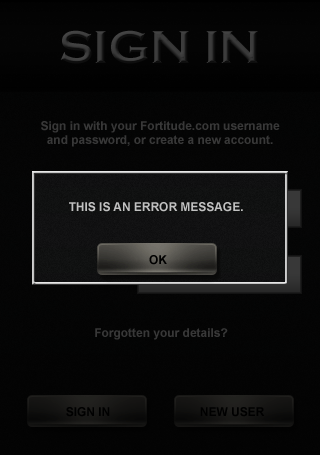
\includegraphics[width=\textwidth]{images/message_box_in_use_mockup}
		\caption{An example of a message box displaying an error message.}
		\label{message_box}
		\end{minipage}
		\end{center}
	\end{minipage}
\end{tabular}
\vspace{-0pt}
\end{figure}

Should the user input invalid information, such as incorrect login details, then an error message will be displayed (see fig 2.21). The screen behind this message will be dimmed to ensure the message is clearly visible. A similar design will be used for all message alerts to the user, such as error messages, status messages (for example `connecting to server') or confirmation messages, which may have two options for the user to choose between (see fig 2.22)

\begin{wrapfigure}{r}{0.25\textwidth}
	\vspace{-20pt}
	\begin{center}
	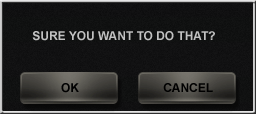
\includegraphics[width=0.25\textwidth]{images/message_box_question_mockup}
	\caption{A message box with two options.}
	\label{message_box_two_options}
	\end{center}
	\vspace{-50pt}
\end{wrapfigure}

Message boxes and text input fields are always of a consistent design to make them easy for the user to identify, though message boxes may stretch to contain longer messages.

\subsubsection{Menu and Information screens}

Many screens in the application give the user a set of options or provide some form of information. Viewing caches is one such example, as is the account menu (fig 2.23). The primary aim of these screens is to make the information as clear as possible to the users while at the same time making efficient use of space, so that the user does not have to click through multiple nested menus to access any feature. There is also consistency across screens; the `cancel' button, for example, is always either the central bottom button or the bottom right.

The use of images when viewing a cache provides not only aesthetic appeal, but also serves a functional purpose. With different images used for enemy caches, allied caches and administrator caches, it is easy to identify from the cache screen what type of cache is being viewed; again, this refers back to requirement 5.2.26: Distinguishing caches.
\newpage
\vspace{-20pt}
\begin{figure}[h!]
\centering
\begin{tabular}{cc}
	\begin{minipage}{0.3\textwidth}
		\begin{center}
		\begin{minipage}{0.83\textwidth}
		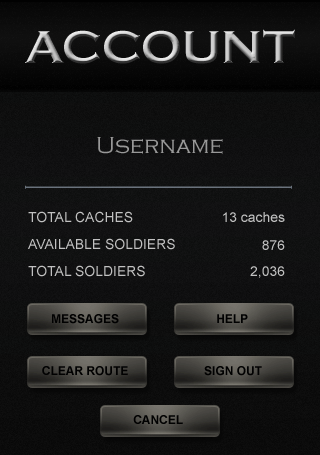
\includegraphics[width=\textwidth]{images/account_mockup}
	\caption{The user's account menu.}
	\label{account}
		\end{minipage}
		\end{center}
	\end{minipage}
	
	\begin{minipage}{0.3\textwidth}
		\begin{center}
		\begin{minipage}{0.83\textwidth}
		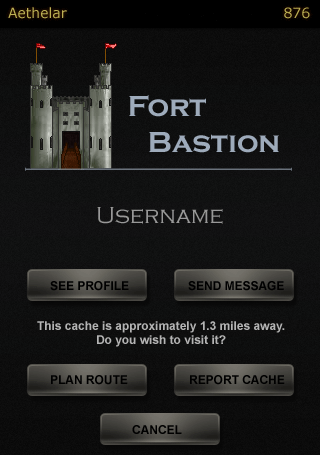
\includegraphics[width=\textwidth]{images/enemy_cache_mockup}
	\caption{Viewing an enemy cache.}
		\end{minipage}
		\end{center}
	\end{minipage}
	\begin{minipage}{0.3\textwidth}
		\begin{center}
		\begin{minipage}{0.83\textwidth}
		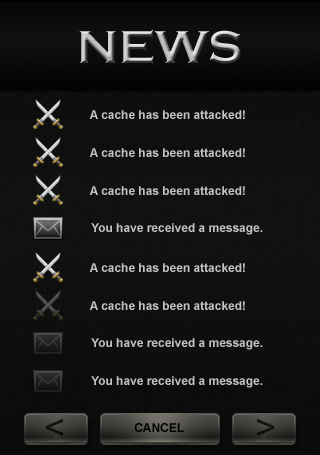
\includegraphics[width=\textwidth]{images/news_mockup}
	\caption{A page of items in the recent news.}
		\end{minipage}
		\end{center}
	\end{minipage}
\end{tabular}
\vspace{-0pt}
\end{figure}

\subsubsection{List screens}

Lists are used for displaying news items and messages in the inbox. Each screen displays several items on a single screen with forward and back buttons at the bottom of the screen to view the next page of items. This helps to limit data usage and loading times for the user whilst also providing an easy to navigate, well ordered system of displaying the items.

The use of icons to distinguish between types of items - battle reports and news icons, for example - makes it easier to take the list as a whole in without difficulty, and fading the icons of items which are not new helps the user find the important information with greater ease (as shown in the bottom 3 icons of fig 2.25).

\subsubsection{Action screens}

\begin{figure}[h!]
\centering
\begin{tabular}{cc}
	\begin{minipage}{0.3\textwidth}
		\begin{center}
		\begin{minipage}{0.83\textwidth}
		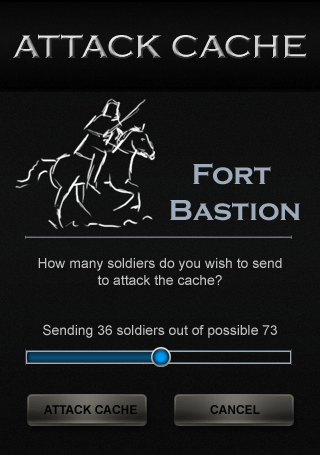
\includegraphics[width=\textwidth]{images/attack_cache_mockup}
	\caption{Attacking a cache.}
		\label{attack_cache}
		\end{minipage}
		\end{center}
	\end{minipage}
	\begin{minipage}{0.3\textwidth}
		\begin{center}
		\begin{minipage}{0.83\textwidth}
		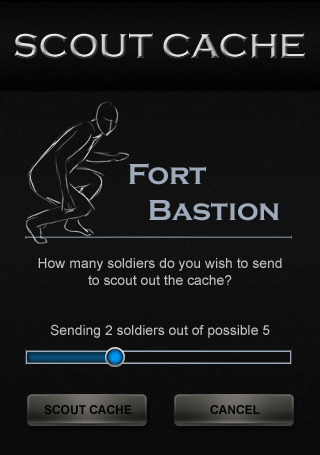
\includegraphics[width=\textwidth]{images/scout_cache_mockup}
	\caption{Scouting a cache.}
		\label{scouting_cache}
		\end{minipage}
		\end{center}
	\end{minipage}
	\begin{minipage}{0.3\textwidth}
		\begin{center}
		\begin{minipage}{0.83\textwidth}
		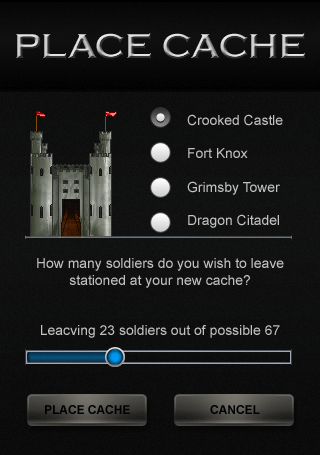
\includegraphics[width=\textwidth]{images/place_cache_mockup}
	\caption{Placing a cache.}
		\label{placing_cache}
		\end{minipage}
		\end{center}
	\end{minipage}
\end{tabular}
\vspace{-0pt}
\end{figure}

 Screens involving direct interaction with caches, such as attacking, managing (withdrawing or depositing soldiers) or placing caches are of a similar layout to provide consistency throughout the game. The screens are clearly differentiated by the use of different images - such as a charging soldier on the attack screen versus a sneaking soldier on the scouting screen (see figs 2.26 and 2.27) as well as by the action title being clearly displayed. The name of the cache involved is also clearly displayed on the screen. Any time that user input is required in these screens it is done in such a way as to restrict the values of possible user input to those which are known to be valid, such as using a slider to change the number of soldiers committed to an action or choosing between a choice of names when creating a cache (see fig 2.28). This is to make the process of game play as quick and error free as possible.

\subsubsection{Reporting results}

Any action with an unknown outcome is reported to the user using a screen of the same design, again to make the app consistent and increase the user's familiarity with how it works and where information is displayed. Where relevant, the image of the report screen reflects the outcome - such as a scroll for a successful scouting mission versus a tomb stone for a failed one (fig 2.29). As ever, this is both for aesthetic reasons and to communicate the necessary information to the user clearly and quickly.

A similar report screen is also accessible from the news feed for the report of a cache the user owns which has been attacked by another player. This screen differs in that the name of the cache is more prominent and there is a link to view the cache on the map; this is required to identify the cache as the user may not be present at the cache's location.

\begin{figure}[h!]
\centering
\begin{tabular}{cc}
	\begin{minipage}{0.3\textwidth}
		\begin{center}
		\begin{minipage}{0.83\textwidth}
		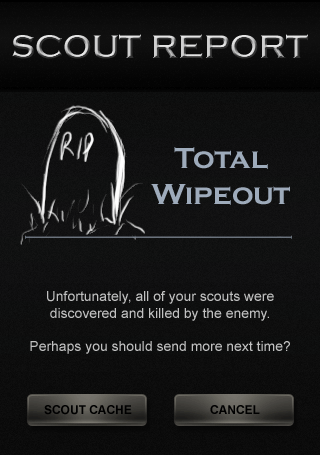
\includegraphics[width=\textwidth]{images/total_wipeout}
	\caption{Unsuccessful scout mission report.}
		\label{attack_cache}
		\end{minipage}
		\end{center}
	\end{minipage}
	\begin{minipage}{0.3\textwidth}
		\begin{center}
		\begin{minipage}{0.83\textwidth}
		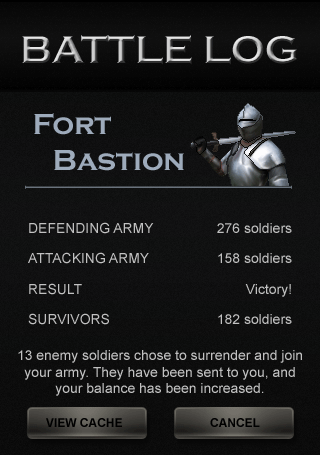
\includegraphics[width=\textwidth]{images/battle_report_mockup}
	\caption{Reporting a battle result.}
		\label{scouting_cache}
		\end{minipage}
		\end{center}
	\end{minipage}
	\begin{minipage}{0.3\textwidth}
		\begin{center}
		\begin{minipage}{0.83\textwidth}
		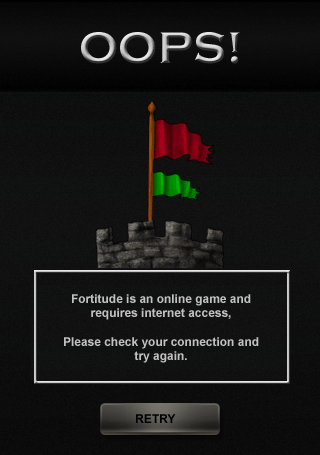
\includegraphics[width=\textwidth]{images/error_mockup}
	\caption{An error caused by lack of internet connection.}
		\end{minipage}
		\end{center}
	\end{minipage}
	
\end{tabular}
\vspace{-0pt}
\end{figure}

\subsubsection{Static screen}

The final type of screen is a static screen. This is one not designed for much user interaction; the full screen is comprised of a single image or static text, such as the Fortitude logo on the splash screen or the help screens (fig 2.1). The splash screen itself has no buttons for the user to progress, as the app will automatically move on once it has loaded. Other static screens, such as the help screens, have a button to move on from this screen.

Static screens are used for errors which cause the app itself to be unplayable - the most common of which would be the user not having internet connection available (see fig 2.31) - and the user will be unable to move from this screen until the error has resolved. A static screen is also used for when a user comes across a special placement cache, with which they cannot interact but must either accept or reject the prize.

With the exception of the help screens, static screens cannot be called by the user; they are initiated by the server and used to send a message to the user that cannot be ignored or minimised until normal game play can resume.

\subsection{User Interface Design - Fortitude-game.co.uk}

\subsubsection{Site Layout}

The visual design of the website was chosen to reflect the dramatic battle-driven nature of the game of Fortitude. It clearly echoes the app in its sombre colour scheme of black, white and greys, and the use of the two flags image used as Fortitude's logo (see fig 2.4). The choice of a more serious design both in the website and the app is to reflect the strategic and `epic' style of game that Fortitude is, appealing to players of all ages.

\begin{wrapfigure}{l}{0.6\textwidth}
	\vspace{-30pt}
	\begin{center}
	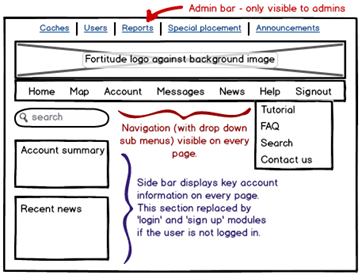
\includegraphics[width=0.6\textwidth]{images/website_wireframe}
	\caption{Wireframe of the site layout with space left for page content. The image used in the header is shown previously in figure ~\ref{fig:website_header} on page~\pageref{fig:website_header}.}
	\label{website_wireframe}
	\end{center}
	\vspace{-20pt}
\end{wrapfigure}

The basic structure of the website is for the page to be divided into three, with the top area containing navigation (including administrator links), the sidebar to the left containing key information and the larger area to the right displaying the page content for each page (see fig 2.32). Both the sidebar to the left and the main page content of the home page use modules to display content, making the information easily and quickly accessible. The administration links have been placed above the main page to ensure that they cannot interfere with the usual page content but are not sidelined and hard to get to; it is anticipated that administrators would mainly use the website for admin purposes, and so need the links to be clearly visible. These links will not be displayed for any user who is not an administrator; should they reach an administrator page, they will be shown a 404 page. Similarly, some pages are restricted to users; should a visitor who is not logged in attempt to view a page such as the account page, they will be redirected to the login/sign up screen.

The use of drop down sub menus is important to increase ease of navigation, enabling users to quickly reach areas of the website without over cluttering the top bar itself. However, as not all devices have a hover feature (such as tablets or phones), no area of the website will only be accessible through these sub menus.

\subsubsection{Site Content}

The content of the website will in many cases mimic that of the app, though in greater depth or with greater functionality - for example, the user can view caches on a map as they can through the phone, but can also apply a filter to display only their own or only enemy caches, as per requirement 5.4.7: Overview Map (see fig 2.33). In addition, some functionality is only available through the website - such as the ability to search for a user or cache by name, or the ability to view an activity log of recent activity associated with that account, specified in requirement 5.3.6: Activity Recording. Certain content, such as the home screen and site news, is visible to all whether logged in or not so as to give potential users a feel for the game and encourage them to sign up and participate. Other areas will redirect the user to the Login page which consists of two modules, one to log in and one to sign up. These modules will also be visible on the side bar at all times unless the user is logged in, in which case the side bar will display key information.

\subsubsection{The Map}

\begin{wrapfigure}{r}{0.6\textwidth}
\vspace{-40pt}
	\begin{center}
	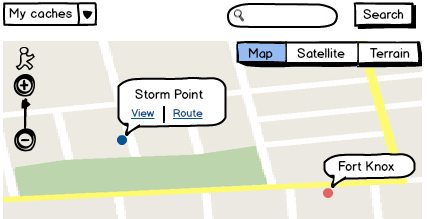
\includegraphics[width=0.6\textwidth]{images/map_wireframe}
	\caption{Wireframe of the map and controls}
	\label{map_wireframe}
	\end{center}
	\vspace{-10pt}
\end{wrapfigure}

The map will use the familiar google maps interface with zoom, street view, and different types of map (satellite, terrain etc). The user can search the map by location, username (ie all caches owned by a certain user) or cache name; should multiple caches with the same name be found, both would be displayed on the map (and the zoom adjusted until both were visible), and the user could zoom in on the correct one. The option to filter caches is done through a drop down menu with filters including `All caches', `My caches', `Enemy caches', and `Outlaw camps' (non-player caches). Updating the map by either filtering or searching is done asynchronously, providing a much smoother experience for the user without having to reload the page each time a request is sent.

\begin{wrapfigure}{l}{0.35\textwidth}
	\vspace{-20pt}
	\begin{center}
	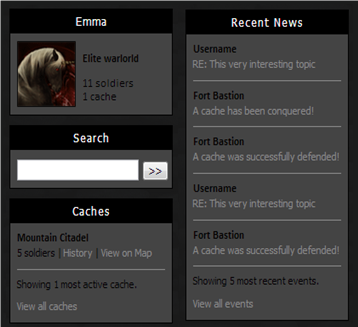
\includegraphics[width=0.35\textwidth]{images/sidebar}
	\caption{The key information displayed in the sidebar (recent news would be placed below rather than beside the other modules).}
	\label{sidebar}
	\end{center}
	\vspace{-80pt}
\end{wrapfigure}

Different types of caches are distinguished as on the app by colour and the presence of a dot, such that colour blind people can also tell caches apart. A cache displays its name and, when clicked on, choices to view the cache details or plan a route to it; this option will bring up a dialogue box asking for the location to plan the route from.

\subsubsection{Sidebar}

As mentioned previously in the Design Methodology (2.1.2), users will in future be able to personalise sections of the website including the sidebar to display the modules most appropriate to them. Until such a point, the sidebar will display to a logged in user a search bar, an account summary, a list of the user's five most active caches - determined by the cache with the greatest frequency of events in its history - and a list of the user's five most recent events. If a user who is not logged in views the site, the sidebar will contain the search module as well as modules to log in or sign up.

The title `Elite Warlord' in fig 2.34 Corresponds to the user's level, determined by the number of caches they own. The avatar and user title serve little purpose as far as game play is concerned, but contribute towards personalising a user's account and, in the levels, giving a tangible goal to aim for in the game.

\subsubsection{Administrator pages}

The administrator features of the website are accessible through the navigation links at the top of the screen, which are only visible to users logged in as administrators. These are highlighted in green, the colour making them stand out and separate from the rest of the website. The tasks that can be completed from each page are shown below in fig 2.36. 
\vspace{55pt}
\begin{figure}[ht]
	\begin{center}
	
\includegraphics[width=0.6\textwidth]{images/admin_bar}
	\caption{The administrator links. The bar itself extends horizontally to fill the page.}
	\label{admin_bar}
	\end{center}
\end{figure}
\begin{figure}[ht]
\begin{center}
\begin{tabular}{| p{0.22\textwidth} | p{0.68\textwidth} |}
	\hline
	Caches &
	View all caches, grouped under `user cache' and `outlaw cache'. Includes options to view the history of or delete caches of any kind or add outlaw caches, as well as managing or editing outlaw caches. \\
	\hline
	Users &
	View the entire user list. Includes options to send users an official warning or other communication and to remove a user account (this would only be done by user request). \\
	\hline
	Reports &
	View all user requests that need to be acted on, and select individual requests to action. \\
	\hline
	Special Placement &
	Create and manage special placement caches. \\
	\hline
	Announcements &
	Post an announcement to the site (appears on the home page and news), and edit or delete old announcements. \\
	\hline
\end{tabular}
\caption {Tasks carried out by admins from each administrator page.}
\label{admin_page_tasks}
\end{center}
\end{figure}


Administrator pages can be roughly grouped into two types; those that involve viewing a database, and those that involve creating data such as a cache, special placement or announcement. Database style pages are laid out as shown in fig 2.37 (the header and sidebar sections are not shown, but are the same as the rest of the site). Filtering the database and commands such as creating new caches or, on the user request page, viewing past requests are linked from the top of the page for easy access, and the database is grouped by a tab system into the types of database. This avoids having redundant fields in an entry - such as the `owner' field for an outlaw camp entry. The administrator cannot ever see the whole database on one page; they are originally shown only the filter section and must access the database by running a query from here. Should the query be too large, the administrator will be requested to narrow down the filter.

\begin{figure}[h!]
	\begin{center}
	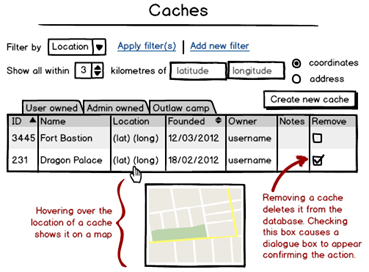
\includegraphics[width=0.6\textwidth]{images/caches_wireframe}
	\caption{Wireframe example of a database page, here managing caches with a location filter selected.}
	\label{caches_wireframe}
	\end{center}
\end{figure}

Creating data is handled through a form interface which, despite its simple design, is arguably the best method of data input for users (Dix, Finlay et al, 1993:105). The form provides user feedback for incorrect or invalid data entries in the same way as creating a user account would (see section 2.1.2).
